\section{Construction and Review Method}\label{sec:method}

\subsection{Design and screening}

A source statement is one recorded practice claim taken from one document. A pattern, called an adopted form once generalization accepts it, is a domain-general rule derived from one or more source statements. A clause is a numbered normative sentence of the Specification. The construction runs in that order, and each step keeps the record of the step before it.

The corpus is practice-first. Engineering practice supplies the candidate rules, because the six failure classes appear in project records long before they appear in papers. The literature enters later, and only to name mechanisms and to bound claims.

Five collection rounds produced 219 source statements. Each round dispatched isolated collectors, twenty in total, and each collector recorded what its assigned sources stated without judging the statement. Filtering was forbidden at this step, so that a later gate could act on a stable population. The orchestrator did not independently refetch every source, so a recording error by a collector survives into the screened population.

Screening then read each of the 219 candidates in isolation. One classifier saw one candidate and one fixed decision block, and saw no other candidate and no running tally. The block asked five questions. Four are hard gates: the statement must generalize beyond its own domain, must strengthen decomposition, contracts, or verification, must preserve human authority over purpose, invariants, risk acceptance, and the definition of done, and must reduce rather than multiply mechanisms. The fifth question assigns a stability class and rejects nothing. Every answer was recorded verbatim, and no answer was later overridden.

The screen kept 113 statements and rejected 106. Of the kept statements, 110 are stable and 3 are volatile. Five rejected statements were then readmitted by a separate and narrower rule: the recorded rejection reason had to name domain specificity as the primary failure, and the statement had to carry a transferable idea that the kept set did not already hold. Each readmission carries its written justification. The two populations stay distinct: 113 statements passed the screen, and 118 statements entered generalization. Figure~\ref{fig:funnel} carries the whole flow.

\begin{figure*}[t]
\centering
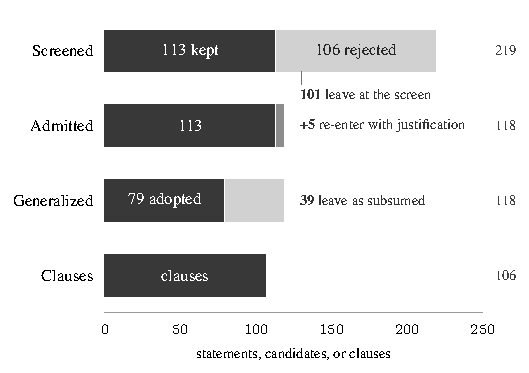
\includegraphics[width=\textwidth]{figures/f01/f01-funnel.pdf}
\caption{The construction funnel. Collection produced 219 source statements. The isolated screen kept 113 and rejected 106. Five rejected statements were readmitted under the secondary rule, giving 118 inputs to generalization. Generalization adopted 79 forms and discarded 39 as subsumed, with none parked. The adopted forms were expressed as 106 numbered clauses; the last row counts clauses, not candidates.}
\label{fig:funnel}
\end{figure*}

The design follows the design-science cycle of \citet{peffers2007}, which builds an artifact against a stated problem and then evaluates it, and it treats practice documents as admissible evidence in the manner of the multivocal review \citep{garousi2019}. The reporting follows the empirical-standards guidance for design-science and methodological work \citep{ralph2021,baltes2026}, and the construction of a method from named, reusable fragments follows method engineering \citep{brinkkemper1996}. Three departures from those frames are recorded. The protocol was not registered before collection. The screening decisions received no independent human validation, and the correction and review passes described below are the substitute. I stopped collection when I judged that the sources supplied no further mechanisms, not when a measured coverage threshold was met.

\subsection{Generalization and correction}

I established the vocabulary used to generalize the 118 candidates in one pass. Isolating each candidate, as the screen did, would have been the consistent choice, and it fails here for a structural reason: the risks of this step are dilution and duplicate mechanisms, and neither is visible from one candidate. The vocabulary was fixed before the first restatement, and software-specific nouns were excluded from every restatement.

Each candidate received the same five-part record: the original form, an abstract mechanism stated without domain-specific nouns, a domain-general restatement, an explicit answer to three tests, and one decision of adopt, discard, or park. The three tests repeat the three substantive gates of the screen, now applied to the restatement rather than to the source: it must still strengthen decomposition, contracts, or verification, must still preserve human authority, and must still reduce rather than multiply mechanisms.

Duplicates were resolved by subsumption rather than by deletion. Where several candidates carried one mechanism, one restatement was adopted as the canonical form, and every other candidate was discarded with an explicit pointer to the form that absorbed it. Distinct facets of a discarded candidate were folded into the canonical restatement when they added force. Decision records show the shape: \hyperlink{gp-60}{GP-60} is the adopted form, six candidates are discarded as subsumed by it alone, and a seventh names it among the forms that absorb it. A discard at this step never reopens the screening decision; it states only that the candidate is not a separate clause.

The pass adopted 79 forms, grouped into 12 mechanism families, discarded 39 as subsumed, and parked none. No candidate carried value that applied to software alone.

Verification then ran as a separate pass with a different model, against 101 distinct source pages. It applied six criteria and two mechanical checks, and it reported findings without editing the file it checked. The pass recorded 58 forms as correct and 21 as needing revision, and failed none. Revision was therefore needed for 21 of the 79 adopted forms at first writing. This observed first-pass defect rate characterizes this execution of the method and should not be interpreted as an estimate of the method's general error rate.

Correction ran after verification and was bound to its findings. All 21 forms were revised. The fixed terminology block grew from 13 to 21 terms, because load-bearing terms had no definition and the relation between specification and contract was not used consistently. Four conflicts between adopted forms were resolved by narrowing exactly one form of each pair, so that no pair was left mutually exclusive. A third model then ran the final check and confirmed that all 21 corrections were present in the file.

Expression as clauses followed. The adopted forms were rewritten as numbered normative sentences with their actor, modality, and object made explicit, which produced the 106 clauses of the Specification. A clause may carry more than one form, and each clause names the forms it carries in its grounds. Section~\ref{sec:standard} states their structure.

Each clause was then reviewed on its own. One reviewer saw one clause and a fixed set of criteria, and wrote one findings report for that clause, with a replacement wording where the criteria were not met. I reviewed every report and every rewrite, and applied the corrections. The reports are committed, one file per clause.

\subsection{Production protocol and source attribution}

The designed evidence policy of the extraction stage is a fail-safe rule, not a majority rule. Two isolated lanes process the same unit under the same pinned prompt, and the unit is accepted only when both lanes return an identical semantic fingerprint. Any disagreement makes the unit abstain and records a classified gap. No arbiter runs, no vote is taken, and no third call is made, so the policy cannot convert a disagreement into an answer.

The fingerprint is computed, not compared by eye. Each lane returns a set of propositions, and each proposition carries its actor, modality, action, target, its precondition and exception trees, and the byte range of the sentence it came from. The trees are normalized first: nested conjunctions and disjunctions flatten, operands sort by their canonical bytes, exact duplicates drop out, and a one-armed operator collapses to its operand. No rule moves an operand across a negation. The set then sorts by a fixed tuple of byte range, actor, modality, action, target, canonical conditions, and source quote, and ordinals are assigned after that sort. The fingerprint is the SHA-256 of the RFC 8785 canonical bytes of the schema version and that sorted set. Confidence, model identity, timestamps, rationales, and run provenance are excluded from the payload. Two lanes therefore agree only when they read the same obligations out of the same bytes, and differences of wording, order, or self-reported confidence neither create agreement nor destroy it.

That policy was calibrated before it was used. A ratified oracle of 21 cases, carrying 37 propositions taken from the Specification with their source byte ranges, fixed the expected output. The lanes ran in isolated sessions with cross-lane access to output prohibited, at temperature 0, seed 0, and one shared prompt hash. Both lanes ran one pinned model in separate sessions. The designed control asks for two independently trained lineages, and the recorded configuration decision permits isolated sessions of one model instead, so the run shows exact agreement between isolated sessions of one model and not agreement between lineages. The calibration compiled all 21 cases and recorded no consensus failure. The policy identifier, the lane pinning, and every hash are written into the result file, and Appendix~\ref{app:repro} states the configuration that the reported results use.

Dual-lane execution approximately doubled model-call cost, and the available budget did not support its use across the full corpus. The two-lane policy governed calibration and did not govern production: of the five model-bound work programmes, one ran under it, and the corpus passes ran under named single-lane policies with layered independent review, with relation extraction under a reviewed policy with adjudication. I recorded the decision to defer the second production lane, with time and budget as the reasons.

The deferral changed no gate. The gate that requires dual-lane consensus across the corpus is still open; no artifact was relabeled to close it. Each single-lane pass carries the identifier of its own evidence policy in the database metadata, so a consumer reads the standing of a number from the artifact rather than from its surroundings. The clause-to-goal pass had a case-by-case delegated review and an independent audit of the frozen responses by a different model family, and the dependency pass had a blind review of every consequential answer, a rule-based adjudication, and seeded negative audits. Exact-fingerprint consensus governed calibration; layered independent review and adjudication governed production. Section~\ref{sec:results} reports every result against the policy that produced it, and no result in this paper is offered as dual-lane evidence.

The division of work is fixed and is the same throughout. AI agents performed collection, classification, extraction, and drafting under written rules. I fixed the rules, reviewed the records, resolved conflicts, and accepted or rejected the text. Delegated classification is treated as instrument output, in line with reported agreement between model and human coders on annotation tasks \citep{pangakis2023}, with the reported risk that model annotation changes the conclusions drawn from it \citep{baumann2025}, and with the reported limits of model judges and of run-to-run determinism \citep{shi2025,norman2026,atil2025}. Authority over purpose, invariants, risk acceptance, and the definition of done stays with the author, which is the same rule the screen applied to its candidates.

A rating scale for source strength was used and then withdrawn after review and failed controls; no score derived from it appears in this paper.

Source attribution follows the same separation. The literature named in Section~\ref{sec:related} entered after derivation, as positioning and as a bound on novelty. Only one work cited as related work also supplied a pattern: ISO/IEC/IEEE 15288, the source of \hyperlink{gp-16}{GP-16}. Every statement in this paper about an external work is bound to a verified citation record with its locator and its permitted use, and no claim exceeds that permitted use, because language models are known to fabricate references \citep{naser2026}. Appendix~\ref{app:sources} holds the two source sets apart and states what each one was used for. Table~\ref{tab:stages} states, for each stage, what entered it, what left it, the control that bounded it, and the artifact that records it.

\begin{table*}[t]
\centering
\caption{The construction stages, with the control that bounded each one and the artifact that records it. Counts are the populations shown in Figure~\ref{fig:funnel}.}
\label{tab:stages}
\begin{tabular}{>{\raggedright\arraybackslash}p{0.88in}>{\raggedright\arraybackslash}p{1.13in}>{\raggedright\arraybackslash}p{1.13in}p{1.56in}>{\raggedright\arraybackslash}p{1.47in}}
\toprule
Stage & Input & Output & Control & Evidence artifact \\
\midrule
Collection & Practice and standards sources, five rounds & 219 source statements & Isolated collectors; filtering forbidden & Collection log \\
\addlinespace
Screening & 219 source statements & 113 kept, 106 rejected & One candidate per classifier; one fixed decision block; four hard gates & Extraction log, with every decision verbatim \\
\addlinespace
Secondary admission & 106 rejected statements & 5 readmitted, giving 118 inputs & Recorded rejection reason must name domain specificity; written justification per case & Phase~3 methodology record \\
\addlinespace
Generalization & 118 candidates & 79 adopted in 12 families, 39 subsumed, 0 parked & One pass, fixed vocabulary, five-part record, three tests, subsumption pointers & Generalized patterns file \\
\addlinespace
Verification & 79 adopted forms & 58 correct, 21 needing revision, 0 failed & Different model; six criteria and two mechanical checks; reporting only, no edits & Verification log \\
\addlinespace
Correction & 21 flagged forms & 21 revised; terminology 13 to 21 terms & Bound to recorded findings; four conflicts resolved by narrowing one form each & Corrected patterns file \\
\addlinespace
Final check & Corrected file & All 21 corrections confirmed present & Third model, independent of verification and correction & Final verification record \\
\addlinespace
Clause expression & 79 adopted forms & 106 numbered clauses & Actor, modality, and object made explicit; every clause names its grounds & The Specification \\
\addlinespace
Clause review & 106 clauses & Corrected clause text & One clause per isolated reviewer; fixed criteria; I reviewed every report and rewrite & One findings report per clause \\
\addlinespace
Extraction & Clause text & Propositions and relations & Named evidence policy per artifact; calibrated fail-safe rule on 21 cases & Machine-readable result files with policy identifiers and hashes \\
\bottomrule
\end{tabular}
\end{table*}
